\documentclass[a4paper,12pt]{article}
\usepackage[utf8]{inputenc}
\usepackage{graphicx}
\usepackage{subcaption}
\usepackage{amsmath}
\usepackage{url}
\usepackage{float}
\usepackage{babel}
\renewcommand{\figurename}{Slika}  % Change "Figure" to "Slika"
\renewcommand{\tablename}{Tabela}

\begin{document}

\begin{titlepage}
    \centering
	\begin{figure}[htbp]
    	\centering
    	
\includegraphics[width=0.4\textwidth]{./logo.png}
	\end{figure}
    { Univerzitet u Beogradu \\ Matematički fakultet\par}
	
    \vfill

    {\Large \textbf{Seminarski rad}\par}

    \vspace{1cm}

    {\Large \textbf{Ocenjivanje broja ljudi na javnom skupu}\par}

    \vfill

    
	
	
	\begin{tabbing}
	\hspace{10cm} \= \hspace{10cm} \= \kill
	\textbf{Mentor:} \>  \textbf{Studenti:} \\
	dr Marija Cuparić \> Lana Matić 143/2021 \\
	Luka Perović \> Anja Milutinović 235/2021 \\
	\> Smer: Informatika
	\end{tabbing}

    \vfill

    \textbf{Datum:} 2024/25

\end{titlepage}
\newpage
\tableofcontents
\newpage
\section{Uvod}

\newpage
\section{Prikupljanje materijala}

Materijali korišćeni u radu prikupljeni su pomoću snimka dobijenog iz drona \cite{drone_video}, izdvajanjem određenih frejmova koji odgovaraju različitim ulicama. Slike su zatim dodatno isečene tako da nema značajnih preklapanja, radi izbegavanja pojavljivanja istih delova na različitim slikama.
Na narednim slikama prikazani su frejmovi izdvojeni iz snimka dronom.

\begin{figure}[H] 
	\centering 
	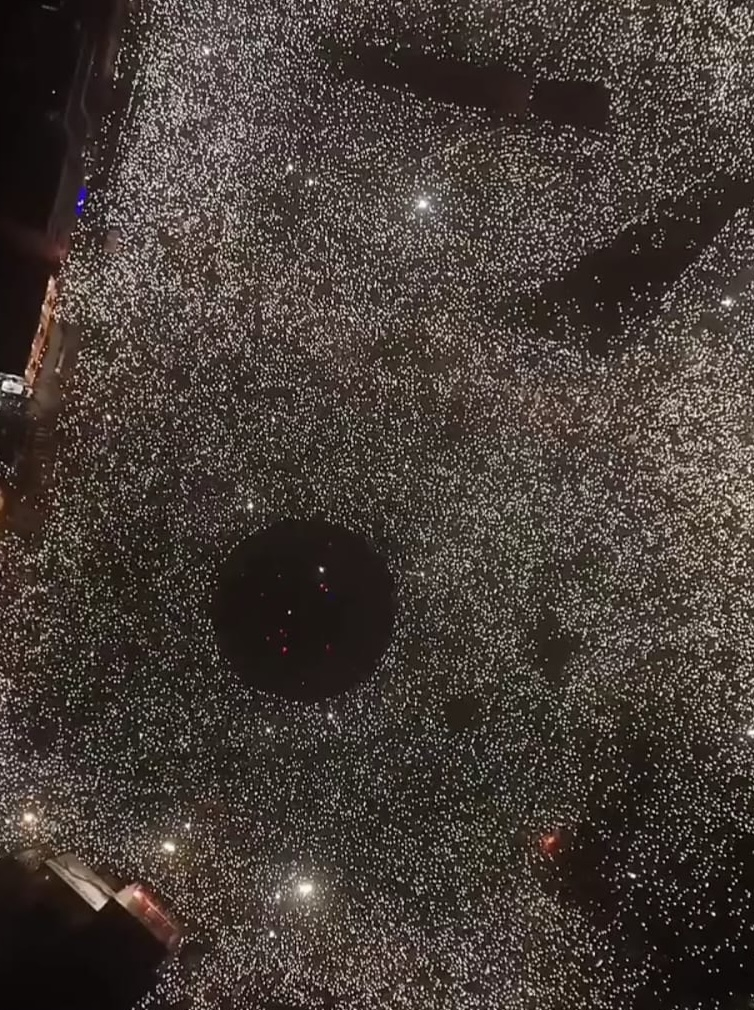
\includegraphics[width=0.8\textwidth]{../images/slavija-centar.jpeg} 
	\caption{Slavija.} 
	\label{fig:slavija} 
\end{figure}

\begin{figure}[H]
	\centering
  
	% Prvi red
	\begin{subfigure}[b]{0.3\textwidth}
	  \centering
	  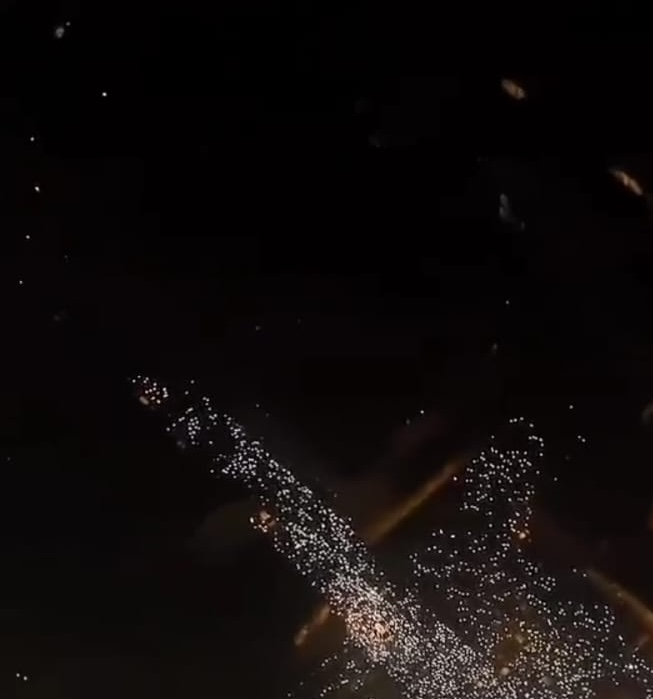
\includegraphics[width=\textwidth]{../images/prote-mateje.jpeg}
	  \caption{Prote Mateje}
	  \label{fig:prote-mateje}
	\end{subfigure}
	\hfill
	\begin{subfigure}[b]{0.3\textwidth}
	  \centering
	  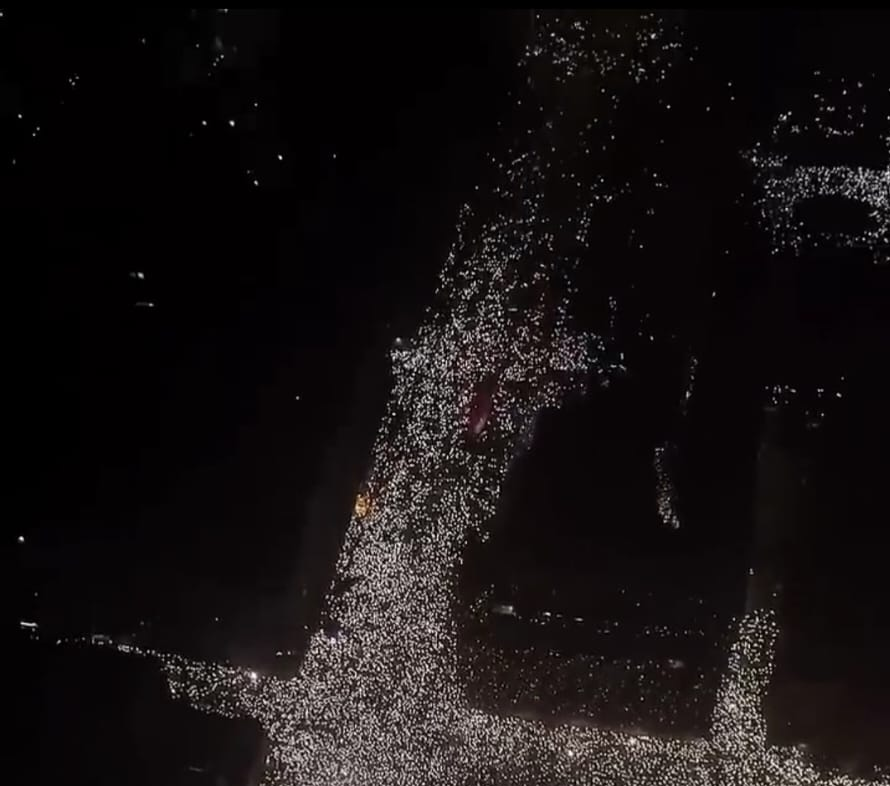
\includegraphics[width=\textwidth]{../images/nemanjina.jpeg}
	  \caption{Nemanjina}
	  \label{fig:nemanjina}
	\end{subfigure}
	\hfill
	\begin{subfigure}[b]{0.3\textwidth}
		\centering
		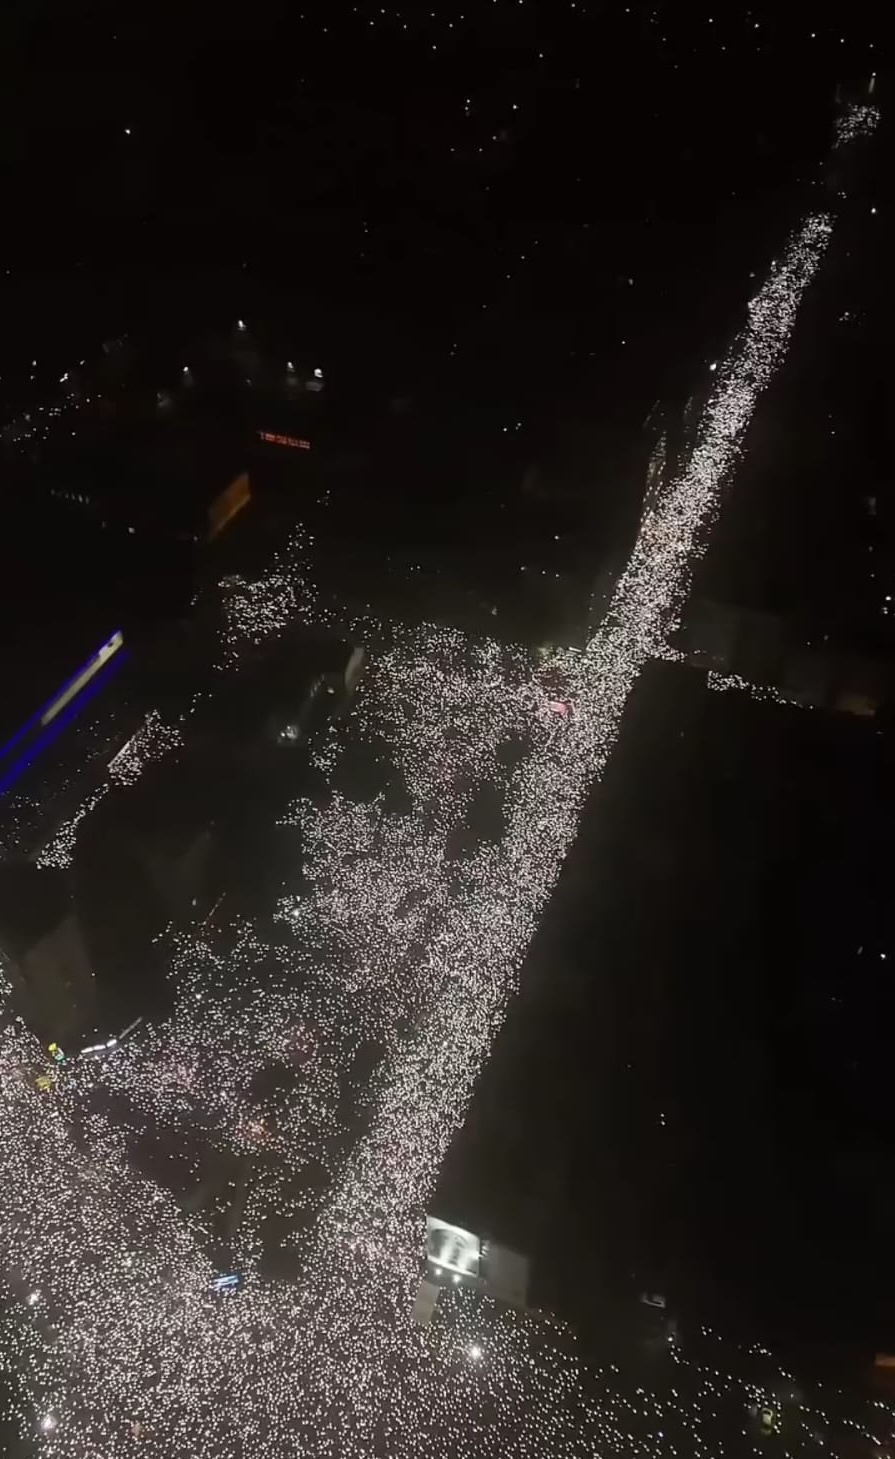
\includegraphics[width=\textwidth]{../images/beogradska.jpeg}
		\caption{Beogradska}
		\label{fig:beogradska}
	\end{subfigure}
  
	\vspace{0.3cm} % razmak između redova
  
	% Drugi red
	\begin{subfigure}[b]{0.3\textwidth}
	  \centering
	  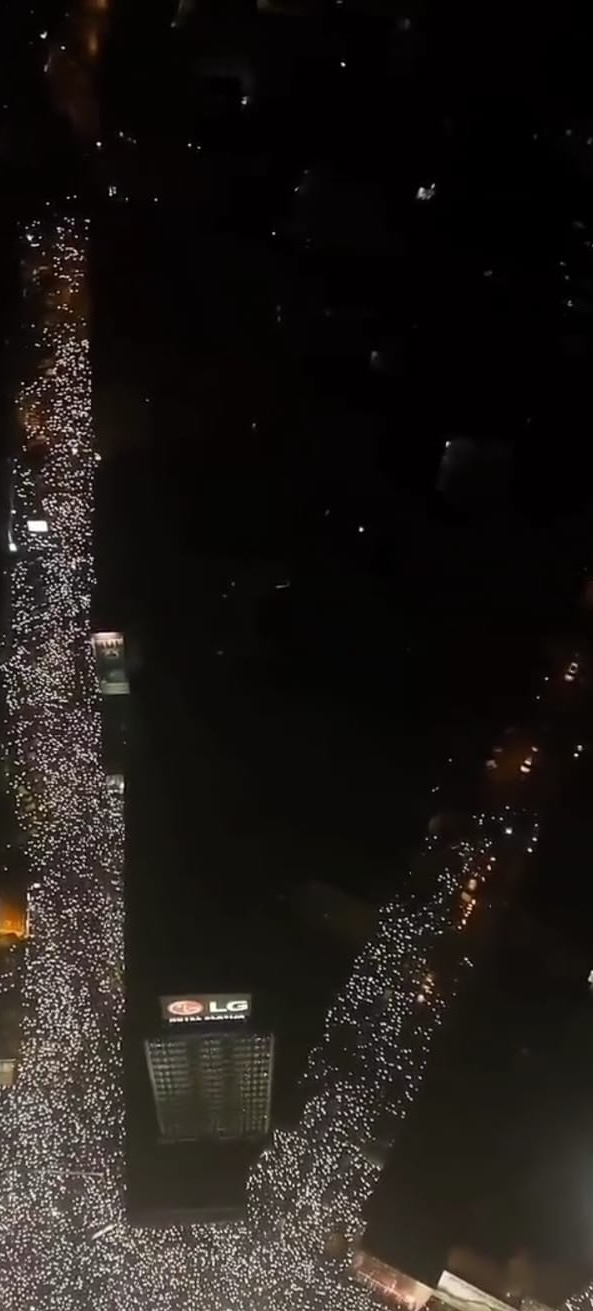
\includegraphics[width=\textwidth]{../images/makenzijeva.jpeg}
	  \caption{Makenzijeva}
	  \label{fig:makenzijeva}
	\end{subfigure}
	\hfill
	\begin{subfigure}[b]{0.3\textwidth}
	  \centering
	  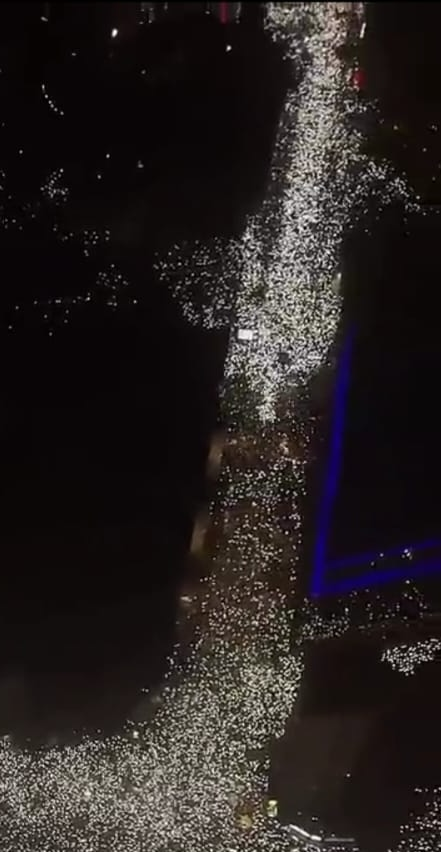
\includegraphics[width=\textwidth]{../images/kralja-milana.jpeg}
	  \caption{Kralja Milana}
	  \label{fig:kralja-milana}
	\end{subfigure}
	\hfill
	\begin{subfigure}[b]{0.3\textwidth}
	  \centering
	  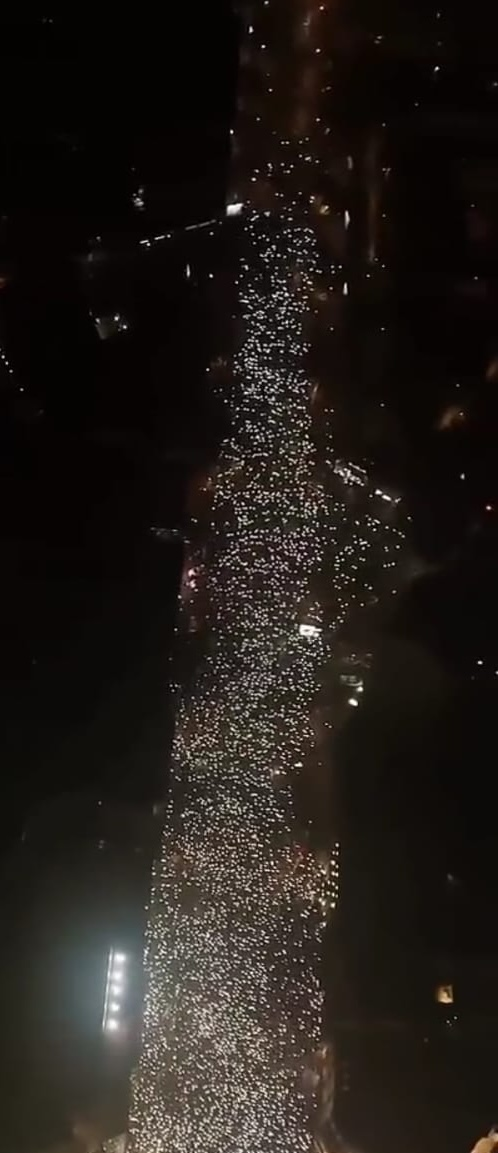
\includegraphics[width=\textwidth]{../images/bulevar-oslobodjenja.jpeg}
	  \caption{Bulevar oslobođenja}
	  \label{fig:bulevar-oslobodjenja}
	\end{subfigure}
  
	\caption{Pregled ulica sa snimka dronom}
\end{figure}




\section{Zaključak}


\newpage
\begin{thebibliography}{9}

	\bibitem{drone_video}
	Autor nepoznat. 
	\textit{Snimak javnog okupljanja dronom}. 
	Dostupno na: \url{https://youtube.com/shorts/4pbj2aZAoP4?si=wxzp9pIkflD2CYKN} 
	(Pristupljeno: 25. septembar 2025.)
	
	\end{thebibliography}

\end{document}